%%%%%%%%%%%%%%%%%%%%%%%%%%%%%%%%%%%%%%%%%%%%%%%%%%%%%%%%%%%%%%%%%%%%%%%%%%%%%%%%
% DisasterSociety — IEEE journal working manuscript
% Rebuilt in the dedicated IEEEtran workspace on 2026-08-14.
% Quantitative results are synchronized from the Carr-S evidence ledger
% (E1 v2 formal, COMPLETE_VALID; E2 v8 formal r7, COMPLETE_VALID;
% E3 v1 cross-model, COMPLETE_VALID; E3a prompt sensitivity v8a/v8b, COMPLETE_VALID;
% E3c scale-100 demonstration, seeds 101/202, COMPLETE_VALID).
%%%%%%%%%%%%%%%%%%%%%%%%%%%%%%%%%%%%%%%%%%%%%%%%%%%%%%%%%%%%%%%%%%%%%%%%%%%%%%%%
\documentclass[journal]{IEEEtran}

\usepackage{amsmath,amssymb}
\usepackage{graphicx}
\usepackage{multirow}
\usepackage{booktabs}
\usepackage{tabularx}
\usepackage{array}
\usepackage{placeins}
\newcolumntype{Y}{>{\raggedright\arraybackslash}X}
\newcolumntype{Z}{>{\centering\arraybackslash}X}
\usepackage{threeparttable}
\usepackage[hidelinks]{hyperref}
\usepackage[nameinlink,noabbrev]{cleveref}
\crefname{figure}{Fig.}{Figs.}
\Crefname{figure}{Fig.}{Figs.}
\crefname{section}{Section}{Sections}
\Crefname{section}{Section}{Sections}
\crefname{table}{Table}{Tables}
\Crefname{table}{Table}{Tables}
\crefname{equation}{Eq.}{Eqs.}
\Crefname{equation}{Eq.}{Eqs.}


\title{DisasterSociety: Generative Agent-Based Simulation of Resident and Household Responses to Dynamic Urban Disasters}

% PENDING(final submission metadata): replace with real authors and affiliations.
\author{Anonymous Author(s)%
\thanks{Author names, affiliations, funding information, and the corresponding
author will be added after the target IEEE journal and review policy are fixed.}}

\markboth{IEEE Transactions Journal Draft, August 2026}%
{Anonymous Author(s): DisasterSociety}

\begin{document}
\maketitle


%%%%%%%%%%%%%%%%%%%%%%%%%%%%%%%%%%%%%%%%%%%%%%%%%%%%%%%%%%%%%%%%%%%%%%%%%%%%%%%%
\begin{abstract}
Urban disaster response is a dynamically coupled social process in which
residents may receive different information, coordinate evacuation plans within
households, and adapt their actions under shared constraints such as roads,
vehicles, and care responsibilities. Generative agents can produce
context-sensitive decisions and communication, while credible social simulation
requires an explicit distinction among residents' private cognition, household
coordination commitments, and authoritative world state. We present
\emph{DisasterSociety}, a generative agent-based social simulation framework
that maintains these states separately and connects them through explicit
message interaction, commitment validation, world arbitration, and execution
feedback. Resident language models observe, remember, plan, communicate, and
propose structured action intentions, while household and world layers determine
whether social agreements and physical actions are valid and executable. In a
Carr-Fire-informed controlled scenario, paired ablations of memory, feedback,
planning, and interaction show that all four mechanisms operate as intended at
their interfaces, whereas only feedback and interaction exhibit consistent
downstream effects. Removing feedback increases closed-route rejections by
6.542 per household; removing interaction eliminates coordinated multi-adult
departure while individual evacuation remains possible. Cross-model and
prompt-wording studies further show that these two mechanism effects are
broadly preserved across decision models and instruction formulations. These
results demonstrate the importance of evaluating both whether a
generative-agent mechanism functions and whether it materially changes
household- and collective-level social behavior.
\end{abstract}

\begin{IEEEkeywords}
Generative agents, multi-agent simulation, urban disaster response, household
coordination, social simulation, event-driven simulation, mechanism ablation.
\end{IEEEkeywords}


%%%%%%%%%%%%%%%%%%%%%%%%%%%%%%%%%%%%%%%%%%%%%%%%%%%%%%%%%%%%%%%%%%%%%%%%%%%%%%%%
\section{Introduction}
Urban disaster response is a temporally evolving social process. Protective-action research shows that residents move through multiple stages, from receiving and interpreting warnings to assessing threats and protective actions and eventually acting under practical constraints \cite{lindell2012padm,mileti1992warnings,huang2012ike,kuligowski2021wildfire,grajdura2021awareness}. These processes also unfold within households and social relationships. Household members may begin in different locations, receive different information, and coordinate gathering, shared-vehicle use, care responsibilities, and departure timing; their responses may ultimately take the form of joint or split evacuation \cite{liu2014uniting,maghelal2017split}.

\begin{figure*}[t]
  \centering
  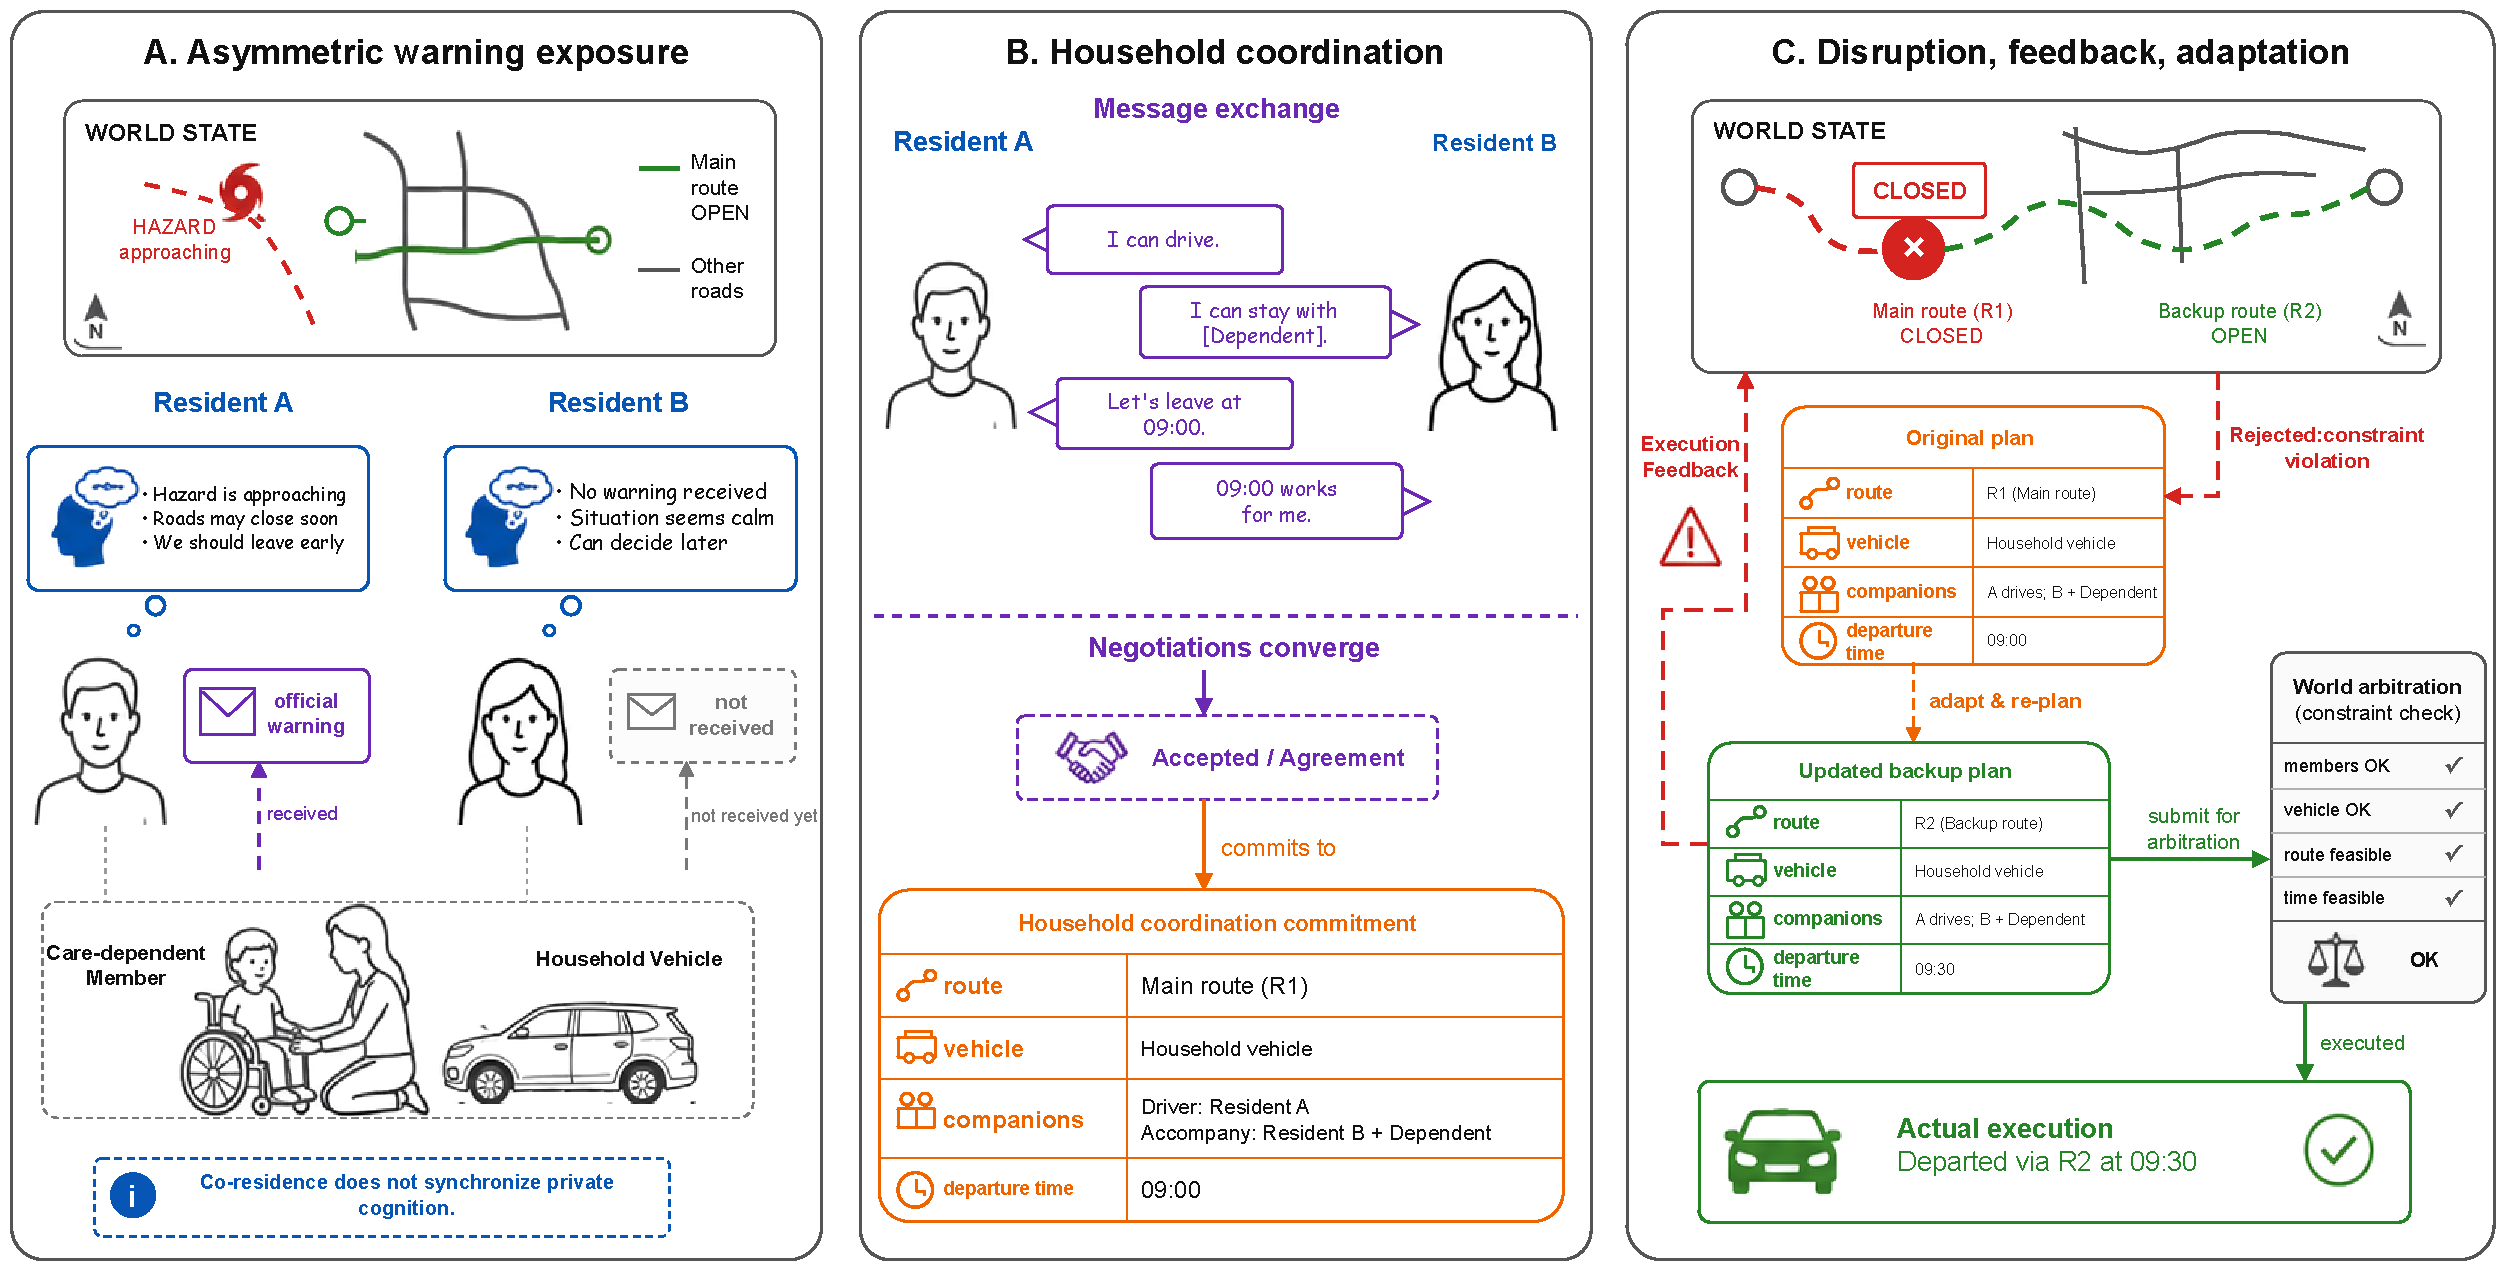
\includegraphics[width=\textwidth]{../figures/fig1_running_example.pdf}
  \caption{Running example of a coupled household evacuation process. (A)
  Asymmetric warning delivery gives co-resident adults different private beliefs
  while the household still shares a vehicle and care responsibility. (B) Message
  exchange converges to a validated household commitment recording route,
  vehicle, companions, and departure time. (C) Closure of the primary route R1
  causes world arbitration to reject the plan; execution feedback triggers
  replanning to the open backup route R2, and the revised action executes. The
  example is Carr-informed and controlled; it illustrates the modeled mechanisms
  rather than reconstructing the historical Carr Fire timeline.}
  \label{fig:running-example}
\end{figure*}

\Cref{fig:running-example} illustrates the type of coupled process considered in this work. Resident A has received an official warning whereas Resident B has not, leaving the two residents with different private cognitions. Through communication, they negotiate a driver, companions, route, and departure time and form a validated household commitment. When the primary route later closes, the original action is rejected by the world, and the execution outcome supports replanning toward the alternate route. This process highlights three requirements for disaster social simulation: representing how information becomes available to individual residents, how household members form shared coordination states, and how socially formed intentions become actions under physical constraints.

Agent-based models provide a bottom-up representation of heterogeneous residents and their interactions, while large language models (LLMs) further support context-sensitive judgment, planning, and natural-language communication. Generative Agents connected memory, reflection, planning, and interaction in a persistent artificial society \cite{park2023generativeagents}, and subsequent work has extended LLM-agent simulation to larger societal and urban settings \cite{zhang2025agentsociety,bougie2025citysim,zhou2026gasim}. Disaster-oriented research now includes theory-informed individual evacuation prediction \cite{chen2025flare}, LLM residents embedded in spatial fire and crowd environments \cite{dang2025fireagents,yang2026whenagents}, and integrated simulations connecting hazards, warnings, and populations \cite{sultimov2026respond}. These developments substantially expand generative resident modeling, while explicit representations of household-level shared coordination and the transition from socially formed intentions to physically executable actions remain limited.

We formulate this challenge in terms of three state boundaries that must be maintained in disaster social simulation: resident-private cognition, household-shared commitments, and authoritative world state. Co-residence does not automatically synchronize warnings, memories, route beliefs, or private plans across household members. A message that has been sent, delivered, or even accepted becomes a household commitment only after member, resource, and timing constraints are satisfied. Likewise, an action intention produced by a language model must be arbitrated against a common physical snapshot before roads, vehicles, locations, and competing resources can be consistently updated. A generative social simulation therefore requires explicit transitions from world information to private cognition, from private proposals to shared coordination, and from shared plans to physical execution.

This leads to the central research question of this paper: \emph{how can LLM-driven residents form information-bounded, traceable, and executable social behavior processes in a dynamic, constrained socio-physical environment?} Information boundedness requires residents to act only on information obtained through permitted observation, delivery, and feedback channels. Traceability requires explicit coordination records connecting private messages to shared household plans. Executability requires every action that may change shared resources or physical state to pass deterministic validation.

To address this question, we present DisasterSociety. The framework maintains resident-private cognition, household-shared state, and authoritative world state separately and connects them through explicit social-interaction and action-execution processes. Resident language models use bounded observations to remember, plan, communicate, and generate structured action intentions. Messages progress through sending, delivery, processing, and response before accepted proposals can become household commitments under explicit constraints. Action intentions are then batch-arbitrated against one authoritative world snapshot, and executed or rejected outcomes are returned to resident cognition. Together, these transitions form a traceable closed loop from private cognition to household coordination and physical execution.

This paper makes three contributions. First, we introduce a state-ownership and execution architecture for generative disaster social simulation that represents resident-private cognition, household-shared constraints and commitments, and authoritative world state as three separately maintained state spaces connected by explicit transitions. Second, we develop a closed social-process model linking communication and action through a coordination chain (sent$\,\to\,$delivered$\,\to\,$processed$\,\to\,$accepted$\,\to\,$feasible commitment) and an execution chain (intention$\,\to\,$world arbitration$\,\to\,$executed/rejected$\,\to\,$feedback), yielding an explicit path from private cognition to household coordination and physical action. Third, we introduce a mechanism-oriented evaluation design that separately tests whether memory, feedback, planning, and interaction operate at their intended interfaces and whether their changes propagate to household- and collective-level outcomes, with paired ablations, cross-model replication, and prompt-wording sensitivity used to assess the stability of the resulting mechanism findings.

The Carr-Fire-informed controlled case serves as the experimental setting for studying these social processes and mechanisms. \Cref{sec:related} reviews related work. \Cref{sec:method} presents the state model, social-coordination mechanisms, and execution process. \Cref{sec:experiments} reports the process, ablation, and robustness studies. \Cref{sec:discussion,sec:conclusion} discuss the findings and their boundaries and conclude the paper.

%%%%%%%%%%%%%%%%%%%%%%%%%%%%%%%%%%%%%%%%%%%%%%%%%%%%%%%%%%%%%%%%%%%%%%%%%%%%%%%%
\section{Related Work}
\label{sec:related}

\subsection{Protective Action and Household Evacuation Behavior}

Protective-action research treats disaster response as a staged process: cues
and warnings must be received, attended to, and understood before threat and
action appraisal, which remain subject to situational impediments
\cite{lindell2012padm,mileti1992warnings,kuligowski2021wildfire}. Warning
exposure, preparation, and departure unfold over time rather than collapsing
into a single binary outcome \cite{grajdura2021awareness}; crisis-informatics
fieldwork shows that official messages reach residents unevenly and are
reinterpreted through social channels before being acted on
\cite{palen2018crisis}. The process is
also social at the household level: members distributed across locations
coordinate gathering and shared-vehicle use, and observed plans do not always
place all members in one departure group
\cite{huang2012ike,liu2014uniting,maghelal2017split}. This literature specifies
which social processes a resident-level model must represent; it does not
dictate a software state machine or establish that an LLM reproduces those
processes.

\subsection{Agent-Based Disaster and Evacuation Simulation}

Classical evacuation modeling is strong where generative cognition is weak.
Dynamic traffic models represent departure-time choice, route choice, and
network assignment at varying behavioral detail
\cite{murraytuite2013overview}, and synthetic-population
pipelines match joint household and person attribute distributions so that
simulated cohorts remain demographically coherent
\cite{beckman1996synthetic,ye2009ipu}.
Belief--desire--intention evacuation models separate belief, intention, and
execution in software, but the resident decision unit is rule-based rather than
generative, and household commitments are not modeled as versioned shared
objects \cite{dawson2012warning}. This literature also supplies the evaluation
standards we adopt: verification and validation as distinct activities
\cite{sargent2013verification,klugl2008validation}, pattern-oriented modeling
\cite{grimm2005pattern}, and transparent documentation
\cite{grimm2020odd}. Recent evacuation-guidance work in this venue varies
scenario difficulty and benchmarks competing controllers
\cite{zhao2025evacrobot}. DisasterSociety is upstream of
network simulators: it produces the departure parties and route intentions a
traffic model would then execute, and does not replace them.

\subsection{Generative-Agent Social Simulation}

Generative Agents combined episodic memory, reflection, planning, and
communication in a persistent artificial community
\cite{park2023generativeagents}.
Subsequent platforms scaled LLM-agent simulation to societal and urban
settings, in some cases through hybrid LLM/numerical designs to control token
cost \cite{zhang2025agentsociety,bougie2025citysim,zhou2026gasim}, and
generative AI has been argued to augment social-science measurement and
simulation alike \cite{bail2024generativeai}. Within this venue, social-network
simulation frameworks formalize how individual behaviors aggregate into
community-level dynamics \cite{rende2025crowd}, and organized multi-agent teams
show that explicit leadership structure reduces communication cost in LLM
cooperation \cite{guo2026embodied}. In the systems
reviewed here, agent communication is often represented without a separately
validated household-level commitment state; an authoritative physical world
that arbitrates whether a linguistically formed plan can execute is rare, and
mechanism-linked ablation of resident cognition is rarer still.

\subsection{LLM Agents in Disaster Response}

LLMs have entered the disaster pipeline at several points. FLARE uses
behavioral theory and LLM reasoning
for individual wildfire evacuation prediction on post-event surveys
\cite{chen2025flare}; Dang et al. embed LLM agents in a cellular-automata fire
environment \cite{dang2025fireagents}; Yang et al. couple LLM decisions with
pedestrian and vehicle evacuation in a dynamic ABM \cite{yang2026whenagents};
and RESPOND joins flood forecasting, alerts, road closures, and population
agents in an integrated demonstration \cite{sultimov2026respond}. Most
recently, hierarchical generative agents organize
one resident's sequential evacuation decisions into three cognition levels and
calibrate against empirical human evacuation data
\cite{mendoza2026hierarchical}. These works organize cognition \emph{within} a
resident; our focus is the complementary boundary \emph{between} residents and
the world---how private cognitions produce household-level coordinated and
physically executable behavior.

Across these lines of work, the unresolved systems question is how to preserve
resident-private information, turn accepted messages into versioned household
commitments, and arbitrate physical execution against one authoritative world
state. DisasterSociety makes these boundaries explicit and evaluates their
mechanisms through controlled ablation (\cref{sec:method,sec:experiments}).


%%%%%%%%%%%%%%%%%%%%%%%%%%%%%%%%%%%%%%%%%%%%%%%%%%%%%%%%%%%%%%%%%%%%%%%%%%%%%%%%
\section{Method}
\label{sec:method}

DisasterSociety is a discrete-time, event-driven generative-agent social
simulation framework for studying how private resident cognition develops into
household coordination and subsequently into physically constrained action
under a changing disaster environment.

The framework maintains three separately owned persistent states:
\emph{resident-private cognition, household-shared state, and authoritative
world state}. Resident language models form cognition, messages, and action
intentions from information available through permitted channels. The household
layer converts socially formed proposals into validated shared commitments,
while the world layer evaluates contemporaneous action intentions against a
common physical snapshot and resolves physical constraints and conflicts.
Execution outcomes are subsequently returned to resident cognition and become
part of the next decision cycle.

This separation assigns information acquisition, social coordination, and
physical execution to explicit state owners and transition processes.
\Cref{fig:architecture} summarizes scenario initialization, the three
persistent states, and the principal transitions connecting them.

\begin{figure*}[t]
  \centering
  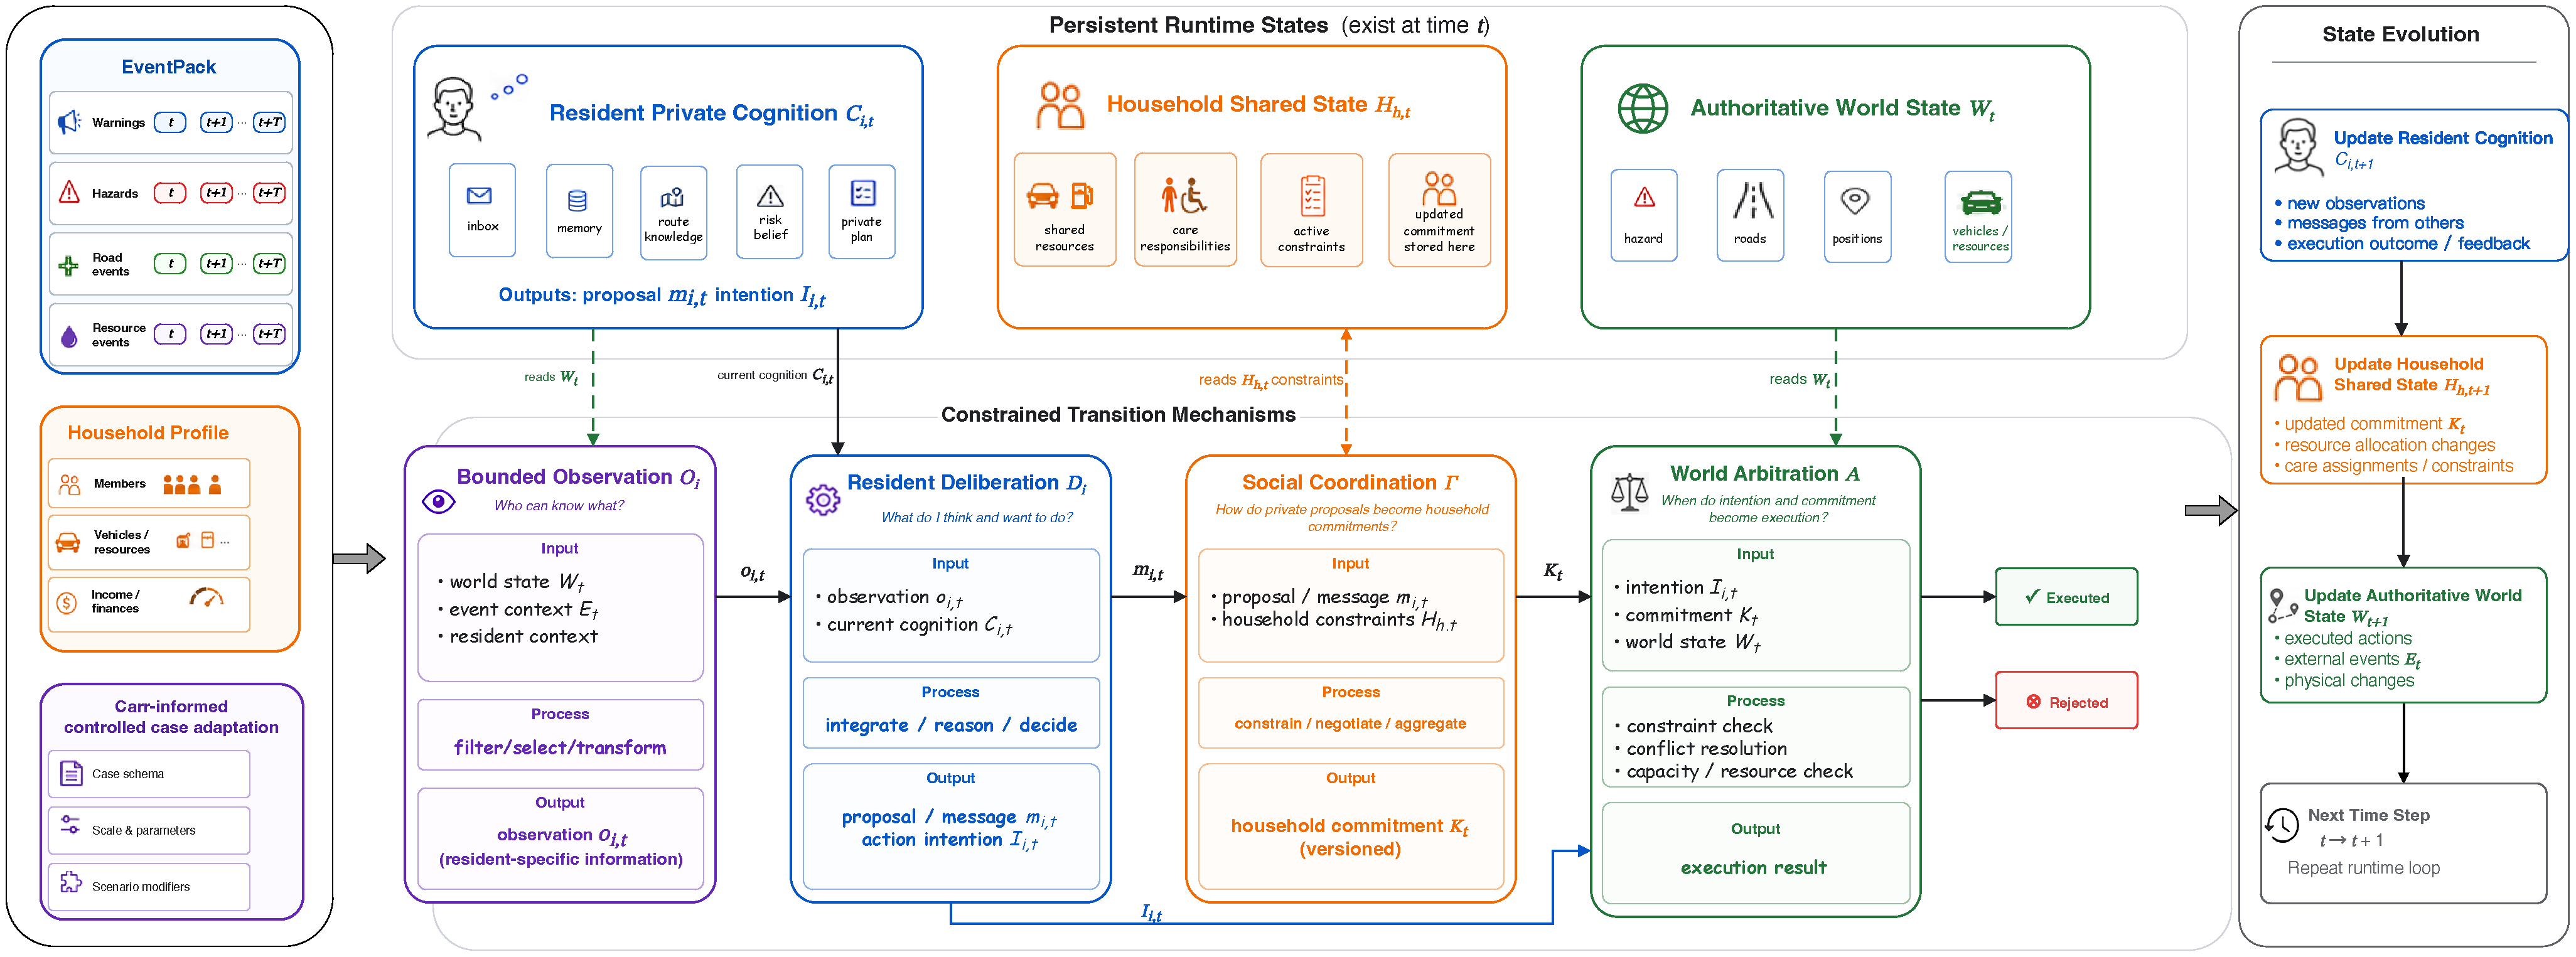
\includegraphics[width=\textwidth]{../figures/fig2_method_framework.pdf}
  \caption{DisasterSociety method framework. Scenario initialization combines a
  time-indexed \emph{EventPack}, a household profile, and controlled case
  adaptation. The runtime maintains resident-private cognition $C_{i,t}$,
  household-shared state $H_{h,t}$, and authoritative world state $W_t$ as
  separate persistent states. Bounded observation converts accessible context
  into resident-specific information $o_{i,t}$; resident deliberation produces
  a proposal or message $m_{i,t}$ and an action intention $I_{i,t}$; social
  coordination validates proposals into a versioned commitment $K_t$; and world
  arbitration resolves $I_{i,t}$ and $K_t$ against $W_t$, yielding an executed
  or rejected result. The updates become $C_{i,t+1}$, $H_{h,t+1}$, and
  $W_{t+1}$ for the next step.}
  \label{fig:architecture}
\end{figure*}

\subsection{State Model and Ownership Boundaries}

Let residents be indexed by $i\in\mathcal{R}$ and households by
$h\in\mathcal{H}$, with household membership defined by $g(i)=h$. At simulation
step $t$, the system state is
\begin{equation}
S_t=
\left(
W_t,
\{C_{i,t}\}_{i\in\mathcal{R}},
\{H_{h,t}\}_{h\in\mathcal{H}},
Q_t
\right),
\label{eq:state}
\end{equation}
where $W_t$ denotes authoritative world state, $C_{i,t}$ denotes the private
cognitive state of resident $i$, $H_{h,t}$ contains the shared resources,
constraints, and accepted coordination state of household $h$, and $Q_t$ stores
auxiliary event, receipt, message, and interaction-process state.

These states have independent ownership. A change to $C_{i,t}$ does not
automatically propagate to another resident $C_{j,t}$. Private beliefs and plans
enter household-shared state only through explicit social-coordination
transitions, and neither household commitments nor private action intentions
can alter physical state before world arbitration.

Consequently, members of the same household may hold different warnings or
route beliefs; an unexpressed private plan does not constitute a household
agreement; and a resident's belief that a road is open does not alter its
authoritative world state.

Resident $i$'s bounded observation at step $t$ is defined as
\begin{equation}
O_{i,t}=
\Omega_i\!\left(W_t,Q_{\leq t};A_{i,t}\right),
\label{eq:observation}
\end{equation}
where $A_{i,t}$ specifies information channels, recipient relationships,
location, and adapter-specific access rules. The resident then produces a
structured action intention
\begin{equation}
I_{i,t}=
\Pi_i\!\left(C_{i,t},O_{i,t};\theta,\phi\right),
\label{eq:intention}
\end{equation}
where $\theta$ denotes the declared decision model and $\phi$ denotes the
enabled cognitive and interaction mechanisms. $I_{i,t}$ represents a behavioral
proposal and does not itself modify household-shared or physical state.

At the implementation level, a \emph{Resident} owns private cognition and
decision state; a \emph{Household} owns membership, vehicles, care
responsibilities, and accepted household commitments; the
\emph{Interaction} layer owns message lifecycle state; and the \emph{World}
owns authoritative hazard, route, location, resource, and physical-arbitration
state.

\subsection{Information-Bounded Cognition and Structured Action Intentions}

Resident decisions follow an explicit information boundary. Each resident may
use only information obtained through permitted observation, message delivery,
household relationships, and execution feedback. Accessible information may
include the resident profile, currently visible household facts, delivered inbox
items, privately perceived hazard and route state, selected private history,
visible household commitments, and recent execution outcomes.

From this information, the language model returns a structured decision
containing an assessment of the current situation, an action selected from a
closed action set, an optional destination, route, vehicle, departure time,
accompanying members, outgoing messages, responses to previously received
messages, and optional memory updates.

Structured outputs are validated for schema and identifier consistency before
entering subsequent social-coordination or world-execution transitions.

\subsection{Social Coordination, Household Commitments, and World Arbitration}
\label{sec:messages-arbitration}

Social interaction is represented through an explicit message lifecycle.
Messages first progress through
$\textit{sent} \to \textit{delivered} \to \textit{processed}$,
and may subsequently enter \textit{accepted} or \textit{rejected} states after
an explicit recipient response.

These lifecycle states correspond to distinct social-process stages. Delivery
determines whether a message enters the recipient's inbox, whereas processing
determines when it becomes part of private history. Sending, receiving, and
accepting therefore have different effects on subsequent cognition and
coordination.

An accepted proposal becomes household-shared coordination state only after
household-level validation. Let $p$ denote a proposal for household $h$ at step
$t$. A household-valid proposal satisfies $\Phi(p,h,t)=1$, with basic conditions
requiring that the named decision members belong to the household, the proposed
vehicle belongs to the household, a route is specified, and the proposed
departure time is no earlier than the current step. Household commitments are
versioned; when a new validated commitment revises an existing one, the previous
version is cancelled while its supersession relation is retained.

A household commitment records social coordination, while physical execution
remains subject to world arbitration. For contemporaneous action intentions, the
World evaluates a common authoritative snapshot $W_t$ and checks route
availability and capacity, vehicle state, resident positions, care requirements,
and competing resource claims.

The world returns either an executed or rejected outcome. Only executed
outcomes may change resident locations or physical resources. Rejected outcomes
leave the corresponding physical state unchanged and retain a rejection reason
that may enter subsequent resident cognition and planning.

DisasterSociety therefore links two processes,
$\textit{message} \to \textit{household commitment}$
and
$\textit{action intention} \to \textit{world arbitration} \to \textit{execution outcome}$.
The first describes how private communication forms household-shared
coordination, and the second describes how socially formed action plans become
physical behavior.

\subsection{Event-Driven Process Loop and State Update}
\label{sec:dynamic-loop}

Each simulation step advances social and physical state through a fixed
sequence. \Cref{fig:dynamic-loop} summarizes the runtime relationship among
resident cognition, message coordination, household commitments, world
arbitration, and feedback.

\begin{figure}[t]
  \centering
  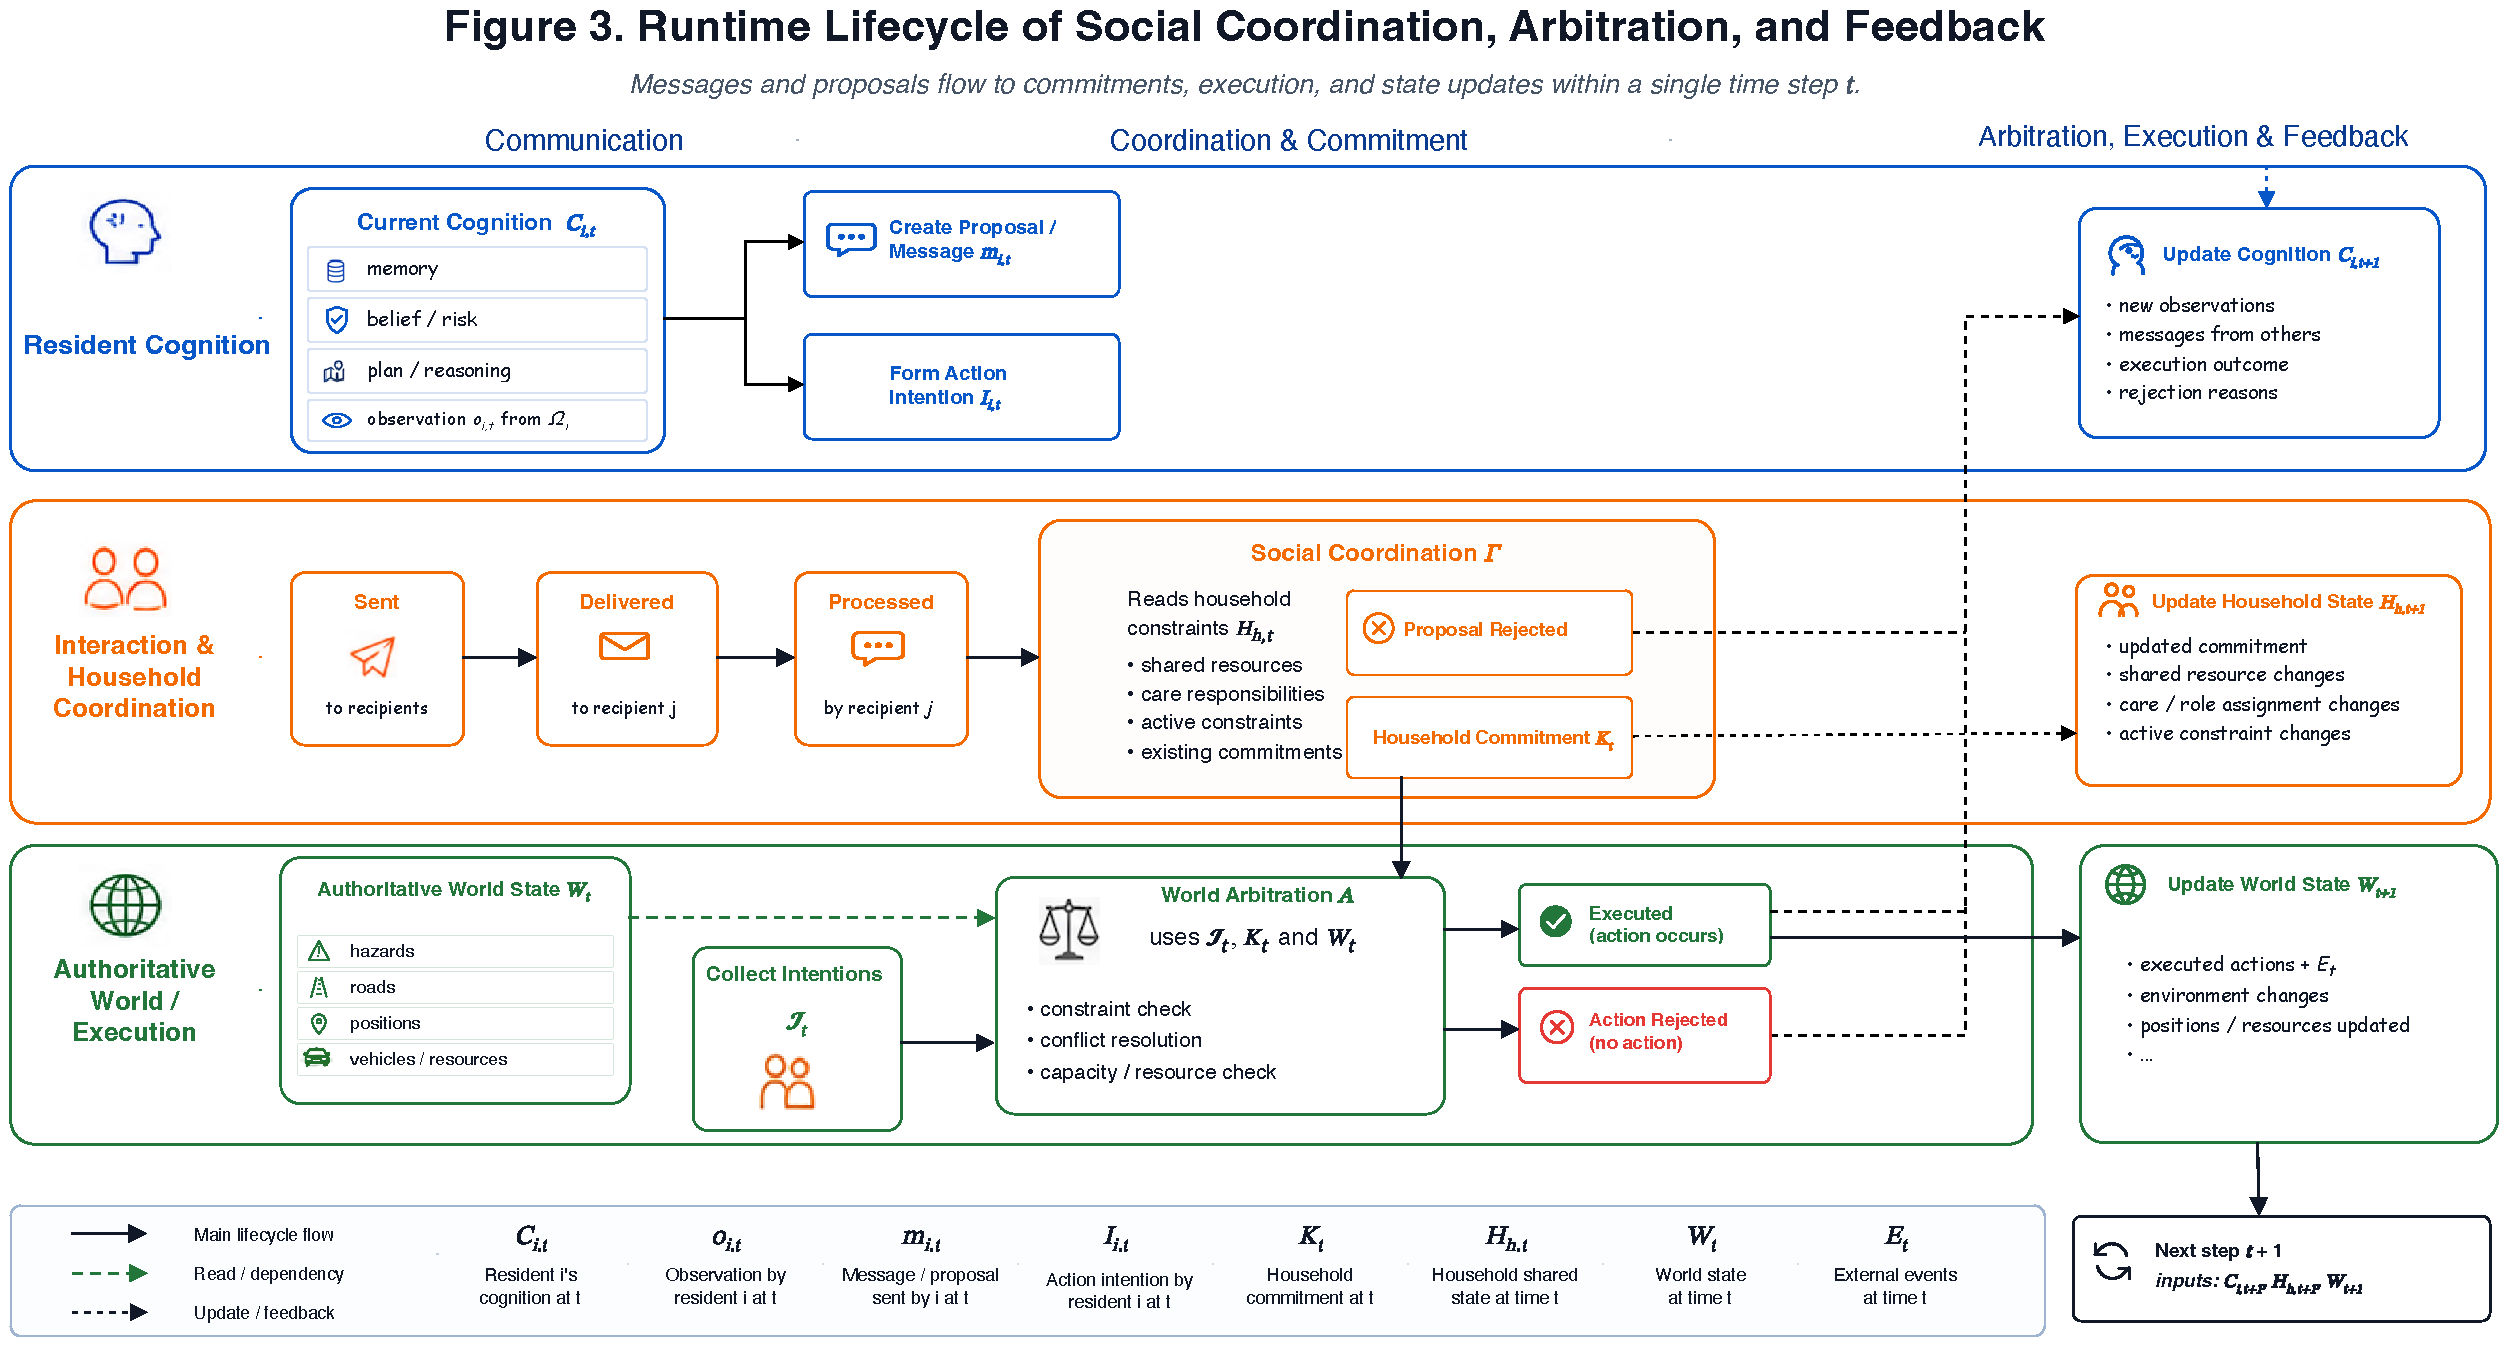
\includegraphics[width=\columnwidth]{../figures/fig3_runtime_lifecycle.pdf}
  \caption{Runtime lifecycle of social coordination, arbitration, and feedback
  within step $t$. Resident cognition produces a proposal or message $m_{i,t}$
  and an action intention $I_{i,t}$. Messages move through sent, delivered, and
  processed states before social coordination either rejects the proposal or
  forms household commitment $K_t$. In parallel, collected intentions,
  commitment $K_t$, and authoritative state $W_t$ enter world arbitration,
  which returns executed or rejected outcomes. Read dependencies and outcome
  feedback produce $C_{i,t+1}$, $H_{h,t+1}$, and $W_{t+1}$ for the next step.}
  \label{fig:dynamic-loop}
\end{figure}

Each step consists of six ordered phases.
(i)~\emph{World advance:} update simulation time, hazard state, and due
exogenous events, and generate associated official warnings or orders.
(ii)~\emph{Wake:} identify residents that require a decision at the current
step. (iii)~\emph{Decision:} solicited residents generate messages and action
intentions in parallel against the same immutable world-state snapshot.
(iv)~\emph{Interaction:} process current inbox items and recipient responses
and update private cognition and household coordination state.
(v)~\emph{Arbitration:} collect contemporaneous action intentions, resolve them
against a common authoritative world state, and return execution outcomes.
(vi)~\emph{Delivery and record:} advance the delivery state of newly emitted
messages and persist the resulting step state and process records.

This ordering ensures that residents act only on information they have obtained,
contemporaneous decisions face a consistent physical environment, rejected
actions do not consume shared resources or change locations, and execution
outcomes can enter cognition, planning, and coordination in subsequent steps.

At the end of the step, resident-private cognition, household-shared state, and
authoritative world state are updated to $C_{i,t+1}$, $H_{h,t+1}$, and
$W_{t+1}$, which jointly provide the state for the next simulation cycle.

\subsection{Scenario and Population Instantiation}

Exogenous disaster processes enter the simulation through an \emph{EventPack}
and scenario adapter. The EventPack organizes warnings, hazard changes, road
events, and resource events, and the scenario adapter converts these inputs into
time-indexed events consumed by the simulation kernel. Authoritative hazard and
road changes are therefore defined by the external scenario.

The experiments use a Carr-Fire-informed controlled scenario. Carr Fire data
provide contextual and provenance constraints. The final fire perimeter serves
as a scenario reference, the two routes are derived experimental assets, and the
road closure is introduced as a controlled perturbation. The resulting world
state may therefore maintain hazard distance, route state and capacity,
resident locations, vehicles, care obligations, and household coordination
commitments.

The resident population is instantiated from weighted household microdata.
Iterative proportional fitting (IPF) adjusts donor-household weights to match
household-level margins for the target area \cite{beckman1996synthetic,ye2009ipu}.
Sampling is then performed at the household level: when a donor household is
selected, its member records are copied together and assigned new synthetic
identifiers. This preserves internally observed relationships such as
co-residence, shared vehicles, and care dependencies.

Initialization maps the sampled population into resident, household-resource,
and care states. Members aged 18 years or older form the transparent
decision-capable baseline, while minors are represented as dependent execution
members. Vehicles maintain household ownership, location, capacity, occupancy,
and reservation state, providing shared-resource constraints for subsequent
household coordination and world arbitration.

\section{Experiments}
\label{sec:experiments}

Three studies instantiate the claim families of our evaluation methodology: an
empirical-process study under the full condition with the richer adapter,
extended by a two-seed scale demonstration at 100 households
(\cref{sec:exp-e1}), the central mechanism ablation with paired
full-versus-removal runs over four mechanism switches (\cref{sec:exp-e2}), and
a bounded cross-model replication of the two determined mechanism effects under
seven decision models, together with an equivalent-prompt sensitivity check on
the same effects (\cref{sec:exp-e3}). All three run the Carr-informed
controlled scenario of \cref{sec:adapters}; none is a historical reconstruction
of the Carr Fire, and no reported quantity is a population-level evacuation
prediction. Existing platforms do not expose matched mechanism controls; we
therefore compare mechanism conditions within one platform, add a
deterministic in-kernel reference policy (\cref{sec:exp-e2}), and replicate
the effects across decision-model families and sizes.

\subsection{Experimental Design and Setup}
\label{sec:evaluation-method}

\subsubsection{Two Experimental Operationalizations}
\label{sec:adapters}

The shared kernel hosts different operationalizations of resident cognition,
and the Carr case uses two adapters with deliberately different estimands
(\cref{tab:adapter-contracts}): one platform, two operationalizations, two
research questions. Both obey the same intention--outcome boundary and state
separation; they differ in cohort construction, private-state representation,
and the claims their artifacts support, and neither operationalization
validates the other's target.

\paragraph{Empirical-process adapter}
This adapter studies a Carr-informed resident process under a full mechanism
configuration with richer donor-microdata trait profiles. Residents are exposed
to a modeled communication substrate (household cliques, nearby neighbors, and
a friend ring---not observed Carr social ties), and coordination takes the form
of structured departure parties whose member, caregiver, vehicle, time, and
overlap checks run at acceptance, with route openness enforced by the world at
execution. A valid solo-adult intention may also form a solo party without
prior negotiation, so the adapter observes coordination where it occurs without
forcing every departure through dialogue; solo parties are reported separately
from multi-adult coordinated departures.

\paragraph{Controlled-mechanism adapter}
This adapter supports paired mechanism identification: conditions share one
household cohort, an initial private primary-route plan, a time-indexed
disruption, and component-isolated exogenous streams, while four code-level
flags enable or remove memory, feedback, planning, and interaction. Its
defining feature for the ablation is the separation of private route perception
from world route truth: with feedback enabled, a decision copies changed world
route state into the private view and rejected execution adds bounded failure
feedback; with feedback disabled, the pre-closure view persists while the world
still arbitrates the true closure. Memory has a deliberately narrow operational
meaning here---delivery-gated warning retention plus model-emitted memory
writes---while the platform's general ranked memory
\cite{park2023generativeagents} remains available through the base resident
interface. The remaining contract differences are summarized in
\cref{tab:adapter-contracts}.

\begin{table*}[tp]
\centering
\scriptsize
\renewcommand{\arraystretch}{0.85}
\setlength{\tabcolsep}{3pt}
\caption{Carr adapter contracts. Both adapters share the kernel, the typed
intention--outcome boundary, and household/world state separation, but differ
in cohort, private-state representation, communication record, and estimand.}
\label{tab:adapter-contracts}
\begin{tabularx}{\textwidth}{@{}p{0.15\textwidth}Y Y@{}}
\toprule
Contract & Empirical-process adapter & Controlled-mechanism adapter \\
\midrule
Purpose and cohort & Carr-informed full-condition process study with richer
PUMS/Carr trait profiles; profile ordering and formal cohort are fixed &
Mechanism identification with seed-selected households containing exactly two
adults, at least one dependent, and exactly one reported vehicle \\
Private cognition & Inbox, recent memory list, perceived routes, private
commitment view, and execution feedback; no persistent executable plan &
Mechanism flags, warning-history signal, feedback-gated route view, executable
plan and plan history, accepted commitments, and recent failure feedback \\
Communication & Recipient-specific official receipts; social messages use a
message-level record over a recipient list and a constructed social graph &
Recipient-specific receipts; household direct and community-audience delivery
are distinct, but the community audience is not a social-network topology \\
Coordination & Structured departure parties with care, vehicle, member, time,
and overlap checks, plus an allowed solo auto-party path & Versioned controlled
household proposals and commitments for the two decision members, with final
execution checks in the world \\
Estimand & Empirical reasonableness and process-constraint correctness;
social-message quantities reported at message level & Paired full-versus-drop-one
mechanism contrasts with manipulation checks and downstream outcomes \\
\bottomrule
\end{tabularx}
\end{table*}

\subsubsection{Reproducibility Infrastructure: Gateway, Seeding, and Run Records}
\label{sec:gateway}

Three properties of the execution infrastructure bear directly on the evidence
reported in \cref{sec:experiments}; the remaining engineering details are
omitted. First, every language-model call passes through a single audited
gateway that enforces schema validation, one repair attempt, and budgets; a
failed call either aborts the run or enters a logged rule fallback that remains
subject to world arbitration, and the fallback share is reported for every run.
Second, controlled-scenario non-LLM randomness is drawn from
component-isolated keyed streams that exclude the experiment condition label,
so paired conditions share exogenous draws and a condition switch cannot
masquerade as a mechanism effect. Third, each run writes step-level world,
intention, outcome, and interaction records and a terminal summary, making
every reported number recomputable from the persisted artifacts.


Evaluation is organized along two orthogonal dimensions. \emph{Analysis scale}
distinguishes individual, household or network, collective, and system
quantities. \emph{Evidence type} distinguishes verification, behavioral
reasonableness, mechanism-specific removal effects, and robustness checks.
This separation follows established simulation methodology
\cite{sargent2013verification,klugl2008validation,grimm2005pattern}; generative
social simulation adds language-model and prompt dependence, motivating
ablations and replication-risk checks
\cite{park2023generativeagents,bail2024generativeai}.

The Carr case uses two non-interchangeable populations. Carr-R is a
version-fixed respondent table for bounded empirical references; Carr-S is a
synthetic household sample for social-process experiments. No survey field is
used both as a run input and as an evaluation target in the same experiment.
Comparisons with Carr-R assess Carr-informed reasonableness rather than
independent validation; the small non-evacuator group and absence of completed
blinded review bound behavioral-validity claims.

For controlled mechanism evaluation, each module has a runner-aligned
manipulation check: memory retains delivered warnings; feedback records a
post-closure alternate-route update among residents with a pre-closure
primary-route plan; planning completes a post-closure alternate-route replan;
interaction forms an all-decision-member commitment referencing the alternate
route, a household vehicle, and a departure step. These are scenario-specific
checks, not general psychological-validity measures. Downstream quantities are
computed from authoritative final state with distinct denominators. The
household-level headline is the \emph{complete safe household departure rate}:
decision-capable members evacuated and dependents safe. Other quantities
include decision-resident evacuation, closed-route rejections, multi-adult
coordinated-departure rate, dependent safety, and shared-resource conflicts.

The controlled contrast for module $m$ and paired seed $s$ is
\begin{equation}
  \Delta_{m,s}=Y_{s,\mathrm{full}}-Y_{s,\mathrm{full}-m},
  \label{eq:ablation}
\end{equation}
a conditional removal effect, not a full factorial decomposition. The run-level
observation is a complete seed$\,\times\,$condition run; paired cells share a
seed and independent replication is across seeds. Seed-level differences are
summarized by
\begin{equation}
  \bar{\Delta}_m=\frac{1}{|S|}\sum_{s\in S}\Delta_{m,s},
  \label{eq:paired-summary}
\end{equation}
with paired-$t$ intervals used only for descriptive visualization in
\cref{fig:e2-effects,fig:e3-cross-model}. Sensitivity is reported through
per-seed direction shares and exact-zero shares.

All model traffic passes through the audited gateway (\cref{sec:gateway}). No
reported cell is excluded: all complete their planned steps with zero failed
calls and zero fallbacks. Every reported quantity is recomputed from archived
per-cell artifacts.

\subsection{Do Households Complete the Response Process End to End?}
\label{sec:exp-e1}

This study exercises the full condition with the empirical-process adapter
(\cref{sec:adapters}): 24 households carrying PUMS/Carr-informed trait
profiles, a constructed social graph, recipient-specific official receipts, and
structured departure parties over 25 steps. Three seeds (7201, 8301, 9401)
complete all planned steps successfully. The decision model is
DeepSeek-V4-Flash, and no call fails or falls back to the rule policy.

\begin{table}[t]
\centering
\footnotesize
\caption{Empirical-process outcomes over 3 seeds (24 households, 25 steps).
Rates are seed means $\pm$ SD; message, commitment, and violation figures are
totals over the three runs. Commitments are reported separately for negotiated
multi-adult commitments and solo auto-parties, which the adapter records as
distinct coordination paths rather than one funnel.}
\label{tab:e1-process}
\begin{tabular}{@{}lc@{}}
\toprule
Quantity & Value \\
\midrule
Complete safe household departure rate & $0.514 \pm 0.024$ \\
Coordinated-departure household rate & $0.333 \pm 0.042$ \\
Split-departure household rate & $0.042 \pm 0.020$ \\
Messages sent $\rightarrow$ deliv.\ $\rightarrow$ processed &
$1214 \rightarrow 710 \rightarrow 665$ \\
Messages accepted / rejected / unanswered & $467\,/\,73\,/\,125$ \\
Departure parties executed (per seed: 10 / 15 / 13) & $38$ \\
Negotiated commitments accepted (all executed) & $15$ \\
Solo auto-parties executed & $23$ \\
Order receipts per run (vol.\ / mand.) & $5\,/\,15$ \\
Care, vehicle, capacity, caregiver violations & $0$ \\
\bottomrule
\end{tabular}
\end{table}

\Cref{tab:e1-process} summarizes the run-level outcomes. Roughly half of the
households reach a complete safe household departure ($0.514 \pm 0.024$ across seeds;
per-seed values 0.500, 0.542, 0.500), one third depart as a coordinated
multi-adult party, and split departures are rare. The message funnel
retains every life-cycle stage---sent, delivered, processed, accepted---so the
lossy channel, not a broadcast assumption, shapes coordination. Execution is
similarly clean: 38 departure parties execute across the three runs with no
party rejected at execution time. The coordination record keeps the two
formation paths distinct: 15 negotiated multi-adult commitments are accepted
and all execute, while the other 23 executed parties are solo auto-parties
formed directly from a valid solo-adult intention without prior negotiation
(\cref{sec:adapters}); neither path records a rejection or cancellation.
Across all
runs, world arbitration records zero care left-behind, vehicle-conflict,
capacity, and caregiver violations: every executed departure party satisfied
the household and resource contracts of \cref{sec:method}.

\paragraph{Distribution-level comparison with the survey reference}
\Cref{tab:e1-dist} places the simulated distributions next to the Carr-R
respondent-sample reference under the estimand alignment of the
reference protocol. The order-to-departure delay is measured identically on
both sides---hours from the first delivered order, mandatory or voluntary, to
the household's first executed departure---and is pooled over the 114
departing order-recipient households across the three 24-household runs and
the two 100-household runs of the scale demonstration below. The simulated CDF
is directionally consistent but compressed: 0.570 of households depart
immediately and 0.868 within thirty minutes, against 0.446 at both grid
points in the survey ($n=186$), and the survey's long right tail (mean 7.1 h;
3.2\% beyond 48 h) has no simulated counterpart. Two structural reasons bound
the comparison: the 25-step scenario window caps observable delays at 12.5 h,
and the half-hour decision cadence resolves each order at the next decision
point, so sub-step hesitation and multi-day delays are outside the modeled
behavior space. Survey channel prevalence
is a multi-select estimand among warned respondents, so we report only
like-for-like prevalence among order recipients rather than first-heard shares
or distribution distances. All 197 simulated recipient households receive the
official direct
channel by cohort construction, and 0.939 also receive at least one
interpersonal (community or intra-household) message, against survey
interpersonal prevalence 0.372 (Wilson 95\% CI [0.312, 0.435]); the survey
splits official receipt across concrete channels (reverse-911 0.359, text
0.380), a taxonomy the scenario collapses into one direct channel. At the
outcome level, the simulated individual departure share is 0.375 over all
members and 0.458 within order-recipient households, well below the survey
evacuation proportion 0.888 (Wilson 95\% CI [0.849, 0.918], $n=330$): unwarned
simulated households rarely self-evacuate, and split parties leave members
behind, whereas the survey estimand is an individual self-report and the
non-evacuator reference group contains only 37 respondents. The study
therefore supports Carr-informed process reasonableness rather than behavioral
validation.

\begin{table}[t]
\centering
\footnotesize
\caption{Distribution-level comparison against the Carr-R
respondent-sample reference. Delays are hours from the first delivered order
to the first executed household departure (simulated: 114 departing
order-recipient households pooled over five runs; survey: $n=186$). Channel
prevalence is multi-select among order recipients (simulated: 197 households;
survey: $n=234$); first-heard and distribution-distance comparisons lack a
matched survey estimand and are not computed.}
\label{tab:e1-dist}
\setlength{\tabcolsep}{4pt}
\begin{tabular}{@{}lcc@{}}
\toprule
Quantity (grid point) & Simulated & Survey reference \\
\midrule
\multicolumn{3}{@{}l}{\emph{Order-to-departure delay CDF}} \\
\hspace{1em}$F(0\,\mathrm{h})$ & 0.570 & 0.446 \\
\hspace{1em}$F(0.5\,\mathrm{h})$ & 0.868 & 0.446 \\
\hspace{1em}$F(1\,\mathrm{h})$ & 0.965 & 0.634 \\
\hspace{1em}$F(2\,\mathrm{h})$ & 1.000 & 0.656 \\
\hspace{1em}$F(5\,\mathrm{h})$ & 1.000 & 0.774 \\
\hspace{1em}$F(12\,\mathrm{h})$ & 1.000 & 0.892 \\
\hspace{1em}Median / mean (h) & 0.0\,/\,0.28 & 1.0\,/\,7.11 \\
\midrule
\multicolumn{3}{@{}l}{\emph{Channel prevalence among order recipients}} \\
\hspace{1em}Official direct & 1.000$^{\dagger}$ & --- \\
\hspace{1em}Any interpersonal & 0.939 & 0.372 \\
\hspace{1em}\quad (survey: reverse-911 / text) & --- & 0.359\,/\,0.380 \\
\midrule
\multicolumn{3}{@{}l}{\emph{Individual departure share}} \\
\hspace{1em}All members & 0.375 & 0.888 \\
\hspace{1em}Order-recipient households & 0.458 & --- \\
\bottomrule
\end{tabular}
\begin{minipage}{\columnwidth}
\vspace{2pt}\scriptsize $^{\dagger}$By cohort construction; the survey splits
official receipt across concrete channels not represented in the scenario.
\end{minipage}
\end{table}

\paragraph{Scale demonstration}
The same protocol is instantiated once more at 100 households---201 members,
153 of them decision-capable residents, receiving 86 official orders---for two
seeds (101, 202) with the same decision model. Both runs
complete all 25 steps successfully. Process behavior carries over qualitatively: complete
safe household departure is 0.470 and 0.420 (against $0.514 \pm 0.024$ at 24
households), coordinated multi-adult departure 0.230 and 0.220, and split departures remain
the minority pattern. The message funnel scales with the population (2,240 and
2,119 messages sent) while preserving every life-cycle stage, and departures
concentrate before the step-9 primary-route closure, with the 11 and 17 later
parties rerouting to the alternate route. Arbitration remains contract-clean at
scale: no executed party violates a care, vehicle, capacity, or caregiver
contract in either run, and the 5 and 6 rejected departure requests (all for
missing traveler intent)
are recorded as rejections rather than executed violations. Within this
demonstrated 100-household envelope we make no larger-size stability or
throughput claim.

\subsection{Which Mechanisms Enable Adaptation After Route Disruption?}
\label{sec:exp-e2}

This study supplies the central mechanism evidence. The
controlled-scenario protocol instantiates the
controlled-mechanism adapter with 8 households---each containing exactly two
decision-capable
adults, at least one dependent, and exactly one vehicle---over 10 steps with a
controlled primary-route closure. Five conditions (the full configuration and
four single-module removals; memory is the bounded warning-retention
operationalization of \cref{sec:adapters}) crossed with 12 seeds give 60
planned cells; all
60 completed. The decision model is DeepSeek-V4-Flash at
high thinking effort, and no call fails, falls back, or is served from cache.
Opportunity is universal for the gating checks: every cell records all 8
households with a warning-exposed coordinator and all 16 decision-capable
members holding a pre-closure primary-route plan, so no manipulation check is
credit-blind.

\begin{figure*}[t]
  \centering
  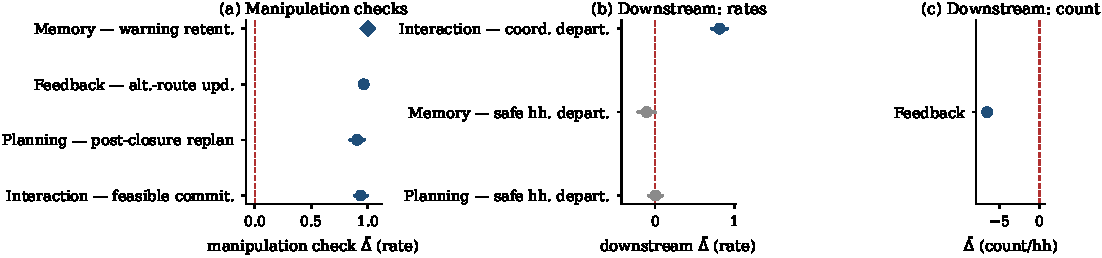
\includegraphics[width=\textwidth]{../figures/fig4_e2_effects.pdf}
  \caption{Paired full-minus-removal contrasts in the ablation study over 12
  seed pairs (points:
  mean paired difference $\bar{\Delta}$; bars: 95\% paired-$t$ intervals).
  (a)~Manipulation checks; the memory check saturates at 1.000 with zero
  variance (diamond). (b)~Downstream rate contrasts; gray marks contrasts
  crossing zero. (c)~The downstream count contrast (closed-route rejections
  per household) on its own scale.}
  \label{fig:e2-effects}
\end{figure*}

\begin{table}[t]
\centering
\footnotesize
\caption{Ablation results over 12 seed pairs, separating mechanism function
(manipulation checks) from downstream necessity (consequences of removal).
$\bar{\Delta}$ is the mean paired full-minus-removal difference; the seeds
column counts pairs whose difference lies in the predeclared direction. A
negative $\bar{\Delta}$ for closed-route rejections means the full condition is
rejected less often. The memory check saturates at its structural
ceiling with zero variance; it verifies that the switch controls the intended
signal rather than estimating a graded behavioral effect.}
\label{tab:e2-ablation}
\begin{tabular}{@{}llcc@{}}
\toprule
Module & Quantity & $\bar{\Delta}$ & Seeds \\
\midrule
\multicolumn{4}{@{}l}{\emph{Manipulation checks (interface function)}} \\
Memory & Warning retention & 1.000 & 12/12 \\
Feedback & Alternate-route update & 0.964 & 12/12 \\
Planning & Post-closure replan & 0.906 & 12/12 \\
Interaction & Feasible commitment & 0.938 & 12/12 \\
\midrule
\multicolumn{4}{@{}l}{\emph{Downstream consequences (necessity)}} \\
Feedback & Closed-route rej./hh & $-$6.542 & 12/12 \\
Interaction & Coord.\ departure & 0.812 & 12/12 \\
Memory & Safe hh.\ departure & $-$0.104 & 2/12 \\
Planning & Safe hh.\ departure & 0.010 & 5/12 \\
\bottomrule
\end{tabular}
\end{table}

\emph{Mechanism function versus downstream necessity.}
\Cref{tab:e2-ablation} separates the two questions the ablation is designed to
distinguish. All four modules pass their interface-level manipulation checks,
each in the predeclared direction for 12/12 seed pairs
(\cref{fig:e2-effects}(a)): memory warning-retention saturates at its structural
ceiling, and the feedback, planning, and interaction checks estimate genuine
behavioral rates of 0.964, 0.906, and 0.938. Only two of the four modules,
however, carry a determined downstream effect (\cref{fig:e2-effects}(b,c)).
Removing feedback raises closed-route rejections by 6.542 per household (12/12
seed pairs): the feedback switch jointly removes route-state refresh and
bounded execution-failure feedback (\cref{sec:adapters}), so the private route
view stays at its pre-closure state and residents repeatedly submit intentions
the world must reject. Removing interaction lowers the coordinated-departure
rate by 0.812 (12/12), and the condition levels give this contrast its precise
meaning (\cref{tab:e2-levels}): half of the decision-capable residents still
evacuate and dependent safety remains 1.000, while execution rejections rise
to 3.833 per household. The interaction mechanism therefore governs the
transition from individual intentions to household-level coordinated action,
rather than evacuation capability itself. In
contrast, the memory and planning contrasts for complete safe household
departure are not determined: $-$0.104 with 2/12 seed pairs in the predicted
direction and 25\% exactly zero, and 0.010 with 5/12 and 17\% exactly zero. The
ablation therefore separates mechanism function from downstream necessity: all
four mechanisms are causally active at their own interfaces, but in an
8-household, 10-step scenario with a single route closure, only feedback and
interaction produce a measurable downstream signature. An undetermined
downstream contrast is not evidence that a module is useless; it bounds what
this scenario can attribute to it.

\begin{table*}[t]
\centering
\scriptsize
\caption{Descriptive condition levels in the ablation study (mean $\pm$ SD over
the 12 cells of
each condition). Safe hh.\ dep.\ is the complete-household safe-departure rate,
which coincides cell by cell with the coordinated-departure rate in this
scenario; resident evac.\ is the decision-resident evacuation rate; rej./hh
denotes rejections per household. Levels are descriptive context for the paired
contrasts of \cref{tab:e2-ablation}, not predeclared contrasts themselves.}
\label{tab:e2-levels}
\begin{tabularx}{\textwidth}{@{}lZZZZZ@{}}
\toprule
Condition & Safe hh.\ dep.\ & Resident evac.\ & Dependent safety &
Closed-route rej./hh & Execution rej./hh \\
\midrule
Full & $0.812 \pm 0.155$ & $0.906 \pm 0.078$ & $1.000 \pm 0.000$ &
$0.000 \pm 0.000$ & $1.198 \pm 0.435$ \\
w/o memory & $0.917 \pm 0.123$ & $0.958 \pm 0.062$ & $1.000 \pm 0.000$ &
$0.000 \pm 0.000$ & $1.073 \pm 0.241$ \\
w/o feedback & $0.021 \pm 0.072$ & $0.042 \pm 0.072$ & $0.055 \pm 0.075$ &
$6.542 \pm 0.671$ & $9.948 \pm 0.880$ \\
w/o planning & $0.802 \pm 0.135$ & $0.901 \pm 0.068$ & $1.000 \pm 0.000$ &
$0.000 \pm 0.000$ & $1.396 \pm 0.455$ \\
w/o interaction & $0.000 \pm 0.000$ & $0.500 \pm 0.000$ & $1.000 \pm 0.000$ &
$0.000 \pm 0.000$ & $3.833 \pm 0.507$ \\
\midrule
Rule reference$^{\dagger}$ & $1.000 \pm 0.000$ & $1.000 \pm 0.000$ &
$1.000 \pm 0.000$ & $0.000 \pm 0.000$ & $1.000 \pm 0.000$ \\
\bottomrule
\end{tabularx}
\begin{minipage}{\textwidth}
\vspace{2pt}\scriptsize $^{\dagger}$Deterministic PADM-style reference policy
on the full condition (same 12 seeds, zero LLM calls): a non-generative
policy-class reference arm, not an ablation condition and not mechanism
evidence.
\end{minipage}
\end{table*}

\emph{Condition levels.} \Cref{tab:e2-levels} reports descriptive condition
levels (means over the 12 cells per condition) as context for the paired
contrasts; they are not themselves predeclared contrasts. Three features stand
out. First, removing feedback does not merely add rejections: complete safe
household departure collapses from 0.812 to 0.021 and dependent safety from
1.000 to 0.055, because households depart on the closed primary route,
accumulate execution rejections (9.948 per household), and never record an
alternate-route update. Second, removing interaction eliminates coordinated
multi-adult departures entirely (0.000 versus 0.812) while exactly half of the
decision-capable residents still evacuate (0.500 with zero variance): the
failure is one of coordination form, not of warning receipt or route knowledge,
both of which remain near ceiling. Third, complete-household safe departure
and coordinated departure coincide cell by cell in this
scenario, so the two
rates measure one process here even though the platform tracks them as distinct
quantities. Memory and planning removal leave levels close to full (0.917 and
0.802 versus 0.812), consistent with their crossing-zero paired contrasts.

\emph{Rule-based reference arm.} To answer what the same scenario produces
without the generative decision model, a deterministic PADM-style reference
policy---warning receipt triggers proposal exchange, a
protective-action commitment, and feedback-driven rerouting to the open
alternate route---was run through the identical kernel, message, and
arbitration pipeline on the full condition for the same 12 seeds, with zero
LLM calls and zero cost. The reference arm reaches the scenario ceiling on
every seed (\cref{tab:e2-levels}), absorbing one transient
route-capacity rejection per household before retrying on a later step. Two
readings follow. First, the scenario is feasible to ceiling, so the generative
full-condition shortfall (0.812 versus 1.000) and the removal collapses above
reflect decision-process degradation rather than scenario hardness. Second,
the ceiling is reached by a policy with exact structured state access and no
language-understanding burden; the arm bounds what a hand-coded policy can
achieve and is a policy-class reference, not mechanism evidence.

\subsection{Do the Mechanism Effects Replicate Across Models and Prompts?}
\label{sec:exp-e3}

This study tests whether the two determined ablation effects are artifacts of a
single decision model. Seven models spanning different families and sizes
(\cref{tab:e3-cross-model}) each run three conditions---full,
full-minus-feedback, and full-minus-interaction---over the same controlled
scenario and prompt on seeds 2107,
2209, 2303, and 2411. Every model completes its 12 cells, giving 28
model--seed pairs pooled; the design is bounded at
four seeds per model and is fully executed.

\begin{figure*}[t]
  \centering
  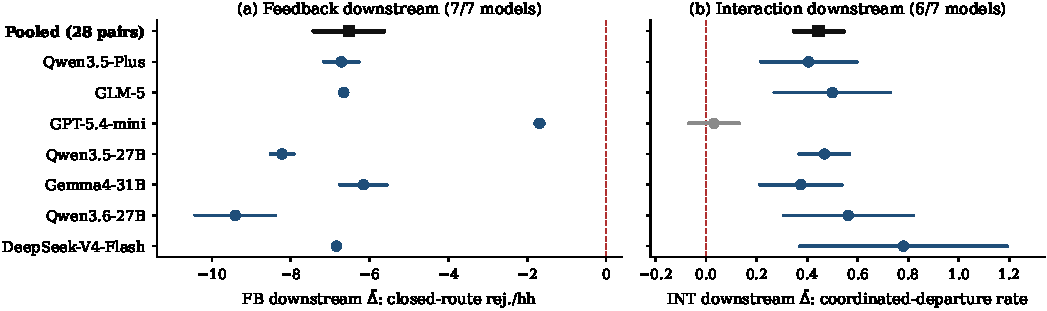
\includegraphics[width=\textwidth]{../figures/fig5_e3_crossmodel.pdf}
  \caption{Cross-model replication of the two determined ablation effects (per
  model: 4 seed pairs; pooled: 28 model--seed pairs; points and bars as in
  \cref{fig:e2-effects}). (a) The feedback downstream effect replicates in
  direction for all seven models. (b) The interaction downstream effect
  replicates for six of seven; GPT-5.4-mini (gray) is the exception.}
  \label{fig:e3-cross-model}
\end{figure*}

\begin{table*}[t]
\centering
\footnotesize
\caption{Cross-model replication of the two determined mechanism effects over
four seeds per model. FB denotes closed-route rejections per household; INT
denotes coordinated-departure rate. Direction reports the seed pairs (of 4)
in the predeclared direction.}
\label{tab:e3-cross-model}
\begin{tabularx}{\textwidth}{@{}lZZZZZ@{}}
\toprule
Decision model & Full safe hh.\ dep.\ & FB: closed rej./hh
(full$\,\to\,$$-$FB) & INT: coord.\ dep.\ (full$\,\to\,$$-$INT) &
Direction (FB$\,\cdot\,$INT) \\
\midrule
Qwen3.5-Plus & 0.406 & $0.00 \to 6.72$ & $0.406 \to 0.000$ & 4/4 $\cdot$ 4/4 \\
GLM-5 & 0.500 & $0.00 \to 6.66$ & $0.500 \to 0.000$ & 4/4 $\cdot$ 4/4 \\
GPT-5.4-mini & 0.031 & $0.00 \to 1.69$ & $0.031 \to 0.000$ & 4/4 $\cdot$ 1/4 \\
Qwen3.5-27B & 0.469 & $0.00 \to 8.22$ & $0.469 \to 0.000$ & 4/4 $\cdot$ 4/4 \\
Gemma4-31B & 0.375 & $0.00 \to 6.16$ & $0.375 \to 0.000$ & 4/4 $\cdot$ 4/4 \\
Qwen3.6-27B & 0.562 & $0.00 \to 9.41$ & $0.562 \to 0.000$ & 4/4 $\cdot$ 4/4 \\
DeepSeek-V4-Flash & 0.781 & $0.00 \to 6.84$ & $0.781 \to 0.000$ & 4/4 $\cdot$ 4/4 \\
\bottomrule
\end{tabularx}
\end{table*}

\Cref{tab:e3-cross-model} reports the replication in terms of condition levels
rather than per-model effect intervals, because the question is whether each
effect's \emph{direction} survives a change of decision model, not which model
scores highest. The feedback effect replicates in direction for every model
(\cref{fig:e3-cross-model}(a)): under the full condition no model records any
closed-route rejection, and removing feedback raises rejections per household
in 4/4 seed pairs for all seven models (from 1.69 for GPT-5.4-mini up to 9.41
for Qwen3.6-27B). The interaction effect replicates in direction for six of
seven (\cref{fig:e3-cross-model}(b)), with removal driving coordinated multi-adult departure
to zero in 4/4 seed pairs for six models. The exception is GPT-5.4-mini (1/4
seed pairs), which runs near the floor in the full condition (complete safe
household departure 0.031, against 0.375--0.781 for the other six models), so
little headroom remains for either removal effect to register a large drop; we
read its interaction contrast as a floor-limited estimand rather than as
evidence against the direction. Full-condition process levels also vary widely
(decision-resident evacuation 0.250--0.891), so the cross-model study supports
the \emph{signs}, not the magnitudes, of the two mechanism effects.

\paragraph{Prompt-wording sensitivity}
A second robustness check varies prompt wording instead of the model. Two
paraphrases of the controlled-scenario prompt---identical state JSON,
schema, mechanism switches, and action set, with only the instruction wording
changed---each run the same four seeds crossed with the same three conditions
(24 cells in all) on DeepSeek-V4-Flash at
temperature 0. Both paraphrases reproduce both determined effects on every
seed pair: the feedback downstream contrast averages $-$7.000 and $-$7.094
closed-route rejections per household under the two variants, against $-$6.844
under the original wording (4/4 seeds in the predicted direction in all three
wordings), and the interaction downstream contrast averages 0.938 and 0.875
coordinated multi-adult departure, against 0.781 (again 4/4 throughout). Manipulation
checks pass in all 24 cells. This check
bounds wording sensitivity within one model family; it
is not evidence of prompt invariance across models or providers.

\section{Discussion}
\label{sec:discussion}

\emph{Mechanism function versus downstream necessity.} The central scientific
finding is the dissociation between the two: all four cognition and
communication modules pass their runner-aligned checks, yet only feedback and
interaction carry determined downstream effects in the controlled scenario, and
the condition levels show them playing different roles---feedback removal is
the only condition that makes dependents unsafe (0.055 versus 1.000), because
the household walks onto the closed route and cannot reroute, whereas
interaction removal leaves every dependent safe but eliminates the coordinated
form. Read at the domain level, the two determined channels are exactly the
ones that cross a state-ownership boundary: feedback reconnects world-state
changes and execution outcomes
to private belief, and interaction converts private intentions into household
coordination. The undetermined memory and planning contrasts admit several
readings---bounded opportunity in a single-closure, 10-step scenario, a
structural rather than graded memory check, or partial substitution that only
a full factorial design could detect. The result suggests a broader evaluation
lesson for
other generative-agent disaster systems
\cite{chen2025flare,dang2025fireagents,yang2026whenagents,sultimov2026respond}:
a mechanism switch validated only at its own interface can overstate necessity
if no downstream estimand is reported;
each switch needs both a manipulation check and a downstream estimand with an
explicit opportunity denominator. Throughout, the platform's contracts held
under full model-driven load, with zero arbitration violations in every
reported run.

\emph{Model dependence.} The directions of both determined effects replicate
across seven models of different families and sizes---feedback in all seven,
interaction downstream in six---while magnitudes vary more than fivefold for
feedback downstream, and full-condition process levels vary more still.
Mechanism-level conclusions about signs are therefore not an artifact of the
ablation's decision model, but per-model quantitative claims remain
model-dependent.

\emph{Boundaries and threats to validity.} All results come from one
Carr-informed controlled scenario archetype---one hazard trajectory, one
controlled closure, 8 households in the ablation and cross-model studies, 24
in the process study, and 100 in the two-seed scale demonstration---and do not
transfer to other hazards, scales, or network structures without new runs.
Carr-R references are directional only: the estimands differ, the
non-evacuator group contains 37 respondents, and both the delay CDF and the
outcome level diverge from the survey (\cref{tab:e1-dist}), so neither is
claimed to be behaviorally validated. The Carr-R test split has been opened for
a feature--outcome diagnostic and no longer serves as an analyst-blind
holdout. No blinded human or expert plausibility review has been
completed, and scenario outputs remain computational artifacts rather than
representations of real persons.

\section{Conclusion}
\label{sec:conclusion}

We presented DisasterSociety, a generative agent-based simulation framework
that separates private resident cognition, household-shared constraints and
commitments, and authoritative world state, connecting them through an
event-driven kernel in which the language model proposes but never mutates
shared or physical state. In a Carr-informed controlled scenario, process
studies at 24 and 100 households completed all runs with zero constraint
violations; a paired twelve-seed ablation showed that memory, feedback,
planning, and interaction each act at their own interfaces, while only
feedback and interaction carry determined downstream effects; and a
seven-model replication with prompt paraphrases reproduced both effect
directions, with one model exception. Ongoing work extends cohort scale,
hazard archetypes, and the cross-model seed count, and adds a prospective
holdout and blinded expert judgment as independent evaluation channels.


%%%%%%%%%%%%%%%%%%%%%%%%%%%%%%%%%%%%%%%%%%%%%%%%%%%%%%%%%%%%%%%%%%%%%%%%%%%%%%%%
\FloatBarrier
{\small
\bibliographystyle{IEEEtran}
\bibliography{references}
}

\end{document}
